\subsection{Object re-use}
\label{sec:object-reuse}

We've already highlighted the importance of memory impact in section \ref{sec:small-nodes} by making the nodes as small as possible. There is another approach we can take to this by making \textit{duplicate} nodes take absolutely no space: we simply re-use existing objects. In this section we will mimic the experiments done by Robin Sedlaczek\parencite{Sedlaczek2015} based on an explanation by Vladimir Sadov\parencite{Sadov2014}. In the end we will have shown how we reach a red-tree façade as shown in image \ref{img:performance-node-reuse-red} while having an underlying structure as shown in image \ref{img:performance-node-reuse-green}.

\begin{figure}[h]
\centering
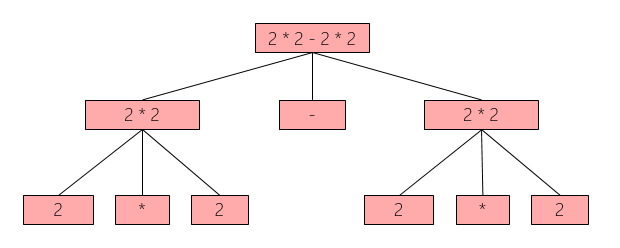
\includegraphics[scale=0.75]{performance-node-reuse-red}
\caption[Red-tree façade]{Red-tree façade \textcopyright Robin Sedlaczek}
\label{img:performance-node-reuse-red}
\end{figure}

\begin{figure}[h]
\centering
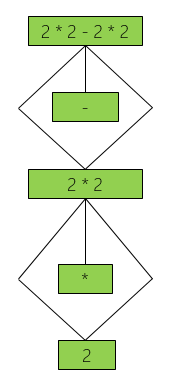
\includegraphics[scale=0.75]{performance-node-reuse-green}
\caption[Underlying green tree nodes]{Underlying green tree nodes \textcopyright Robin Sedlaczek}
\label{img:performance-node-reuse-green}
\end{figure}

\subsubsection{Re-using nodes}
\label{sec:re-use-nodes}

The first aspect we will look at is re-using our green nodes. As we established in section \ref{sec:rg-trees-solution}, green nodes have "vague" information: instead of a specific location in the syntax tree they instead contain the width of themselves. This is good because if it would have a specific location, we would (almost) never be able to re-use it: two distinct nodes in a single tree will be located at a different position. However by using the width instead we \textit{can} consider two similar nodes as identical because we merely look at their width which is the same for both.

We can demonstrate this in the following example where we look at the node that represents \verb|2 + 2|.

\lstset{style=csharp, caption={Re-using nodes based on width vs position}}
\begin{lstlisting}
int x = 2 + 2; // Width: 5; Position: 9
int y = 2 + 2; // Width: 5; Position: 23
\end{lstlisting}

Following out of this and the fact that green nodes don't contain any other uniquely identifying information such as a parent, we can conclude that a single green node can represent multiple identical subtrees. In order to see how this is implemented we have to take a look at the \verb|SyntaxNodeCache|\footnote{\url{https://github.com/dotnet/roslyn/blob/b908b05b41d3adc3b5e81f8cf2d0055c13e4a1f6/src/Compilers/CSharp/Portable/Syntax/InternalSyntax/SyntaxNodeCache.cs}}.

There are three main conclusions that we can take away from this implementation:

\begin{itemize}

\item Limited cache size

Only a limited amount of nodes is stored in this cache. A trade-off has to be made between execution time and memory impact and the Roslyn team has decided to use a cache size of 65536 items (\verb|1 << 16|) as evidenced here:

\lstset{style=csharp, caption={Definition of the SyntaxNodeCache's size}}
\begin{lstlisting}
private const int CacheSizeBits = 16;
private const int CacheSize = 1 << CacheSizeBits;
private const int CacheMask = CacheSize - 1;
\end{lstlisting}

\item First In, First out

When a node is added, a hash key will be calculated. As is typical with hash implementations, this should strive to reach a uniform distribution across the data structure (an array in this case) for optimal performance. Based on this hash key and the mask, the to-be-cached node will be inserted at a certain location of the array. If an entry already exists at this location it will be overwritten, hence the FIFO (First In, First Out) principle.

\lstset{style=csharp, caption={Inserting a node using FIFO}}
\begin{lstlisting}
var idx = hash & CacheMask;
s_cache[idx] = new Entry(hash, node);
\end{lstlisting}

\item Up to 3 children

The last important aspect of this cache is the fact that every node can only have up to three children. If it has any more, the chance of a cache miss is too big\parencite{Sadov2014} so these are not allowed in the first place. This is enforced by making sure there are only overloads available for 1, 2 and 3 nodes.

\lstset{style=csharp, caption={Caching up to three children}}
\begin{lstlisting}
private static bool CanBeCached(GreenNode child1)
{
	return 	child1 == null || child1.IsCacheable;
}

private static bool CanBeCached(GreenNode child1, 
																GreenNode child2)
{
	return 	CanBeCached(child1) && 
					CanBeCached(child2);
}

private static bool CanBeCached(GreenNode child1, 
																GreenNode child2, 
																GreenNode child3)
{
	return 	CanBeCached(child1) && 
					CanBeCached(child2) && 
					CanBeCached(child3);
}
\end{lstlisting}

\end{itemize}

\subsubsection{Re-using tokens}
\label{sec:re-use-tokens}

Tokens are also cached but take a slightly different approach to doing so. When the source text is being parsed, the \verb|QuickScanner| looks inside the \verb|LexerCache| which maintains caches for both trivia and tokens.

\lstset{style=csharp, caption={QuickScanner.QuickScanSyntaxToken}}
\begin{lstlisting}
if (state == QuickScanState.Done)
{
	// this is a good token!
	var token = _cache.LookupToken(
	    TextWindow.CharacterWindow,
	    TextWindow.LexemeRelativeStart,
	    i - TextWindow.LexemeRelativeStart,
	    hashCode,
	    _createQuickTokenFunction);
	return token;
}
\end{lstlisting}

Inside the \verb|LexerCache| the caches for trivia and tokens are stored by way of a \verb|TextKeyedCache| implementation. A \verb|TextKeyedCache| maintains two levels of caching: a local one and a shared one, each with their own characteristics.

\noindent L1 Cache:

\begin{itemize}
\item Small cache size ($2^{11}$ items)
\item Fast
\item Thread-unsafe
\item Local to the parsing session
\end{itemize}

\noindent L2 Cache:

\begin{itemize}
\item Larger cache size ($2^{16}$ items)
\item Slower
\item Thread-safe
\item Shared between all parsing sessions
\end{itemize}

\noindent When an item is searched for in the cache, the \verb|TextKeyedCache| will first attempt to find it in the local cache (\verb|_localTable|) and if it wasn't found there, look in the shared cache (\verb|s_sharedTable|).

\lstset{style=csharp, caption={TextKeyedCache.FindItem}}
\begin{lstlisting}
internal T FindItem(char[] chars, 
										int start, 
										int len, 
										int hashCode)
{
	var idx = LocalIdxFromHash(hashCode);
	var text = _localTable[idx].Text;

	if (text != null && arr[idx].HashCode == hashCode)
	{
		if (StringTable.TextEquals(	text, 
																chars, 
																start, 
																len))
		{
			// Return from local cache
		}
	}

	SharedEntryValue e = FindSharedEntry(	chars, 
																				start, 
																				len, 
																				hashCode);
	if (e != null)
	{
		// Return from shared cache
	}
}
\end{lstlisting}

\subsubsection{Measurements}
\label{sec:re-use-measurements}

In order to visualize the impact of this approach, we will look at three scenarios of syntax tree parsing and see how they affect the heap in terms of object allocation.

\begin{itemize}
\item \textbf{Scenario 1:} Parsing two identical syntax trees

\textbf{Expectation:} When the first tree is created, there will be a relatively large allocation which comes from the green nodes, trivial red nodes and the tokens. Since all nodes and tokens should be re-used, we expect only very minimal overhead that comes from creating the second syntax tree object itself.

\textbf{Demonstration:} 

\lstset{style=csharp, caption={Parsing two identical syntax trees}}
\begin{lstlisting}
internal class Experiment1
{
	public const string tree1 = @"
using System;
using System.Text;

class MyClass 
{
    void MyMethod()
    {
        int result = 2 + 2;
        Console.WriteLine(result);
    }
}";
	private static void Main(string[] args)
	{
		var obj1 = CSharpSyntaxTree.ParseText(tree1);
		var obj2 = CSharpSyntaxTree.ParseText(tree1);
	}
}
\end{lstlisting}

\textbf{Results:}

\begin{figure}[H]
\centering
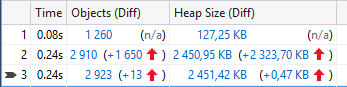
\includegraphics[scale=1]{performance-node-reuse-scenario1-1}
\caption{Memory impact comparison when parsing two identical syntax trees}
\label{img:performance-node-reuse-scenario1-1}
\end{figure}

\begin{figure}[H]
\centering
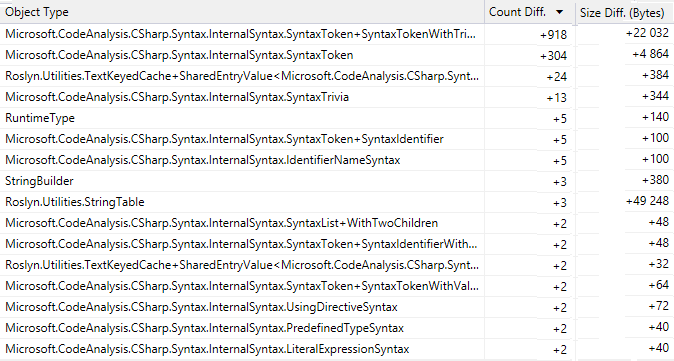
\includegraphics[scale=0.80]{performance-node-reuse-scenario1-2}
\caption{Memory impact of the first parsing session with identical trees}
\label{img:performance-node-reuse-scenario1-2}
\end{figure}

\begin{figure}[H]
\centering
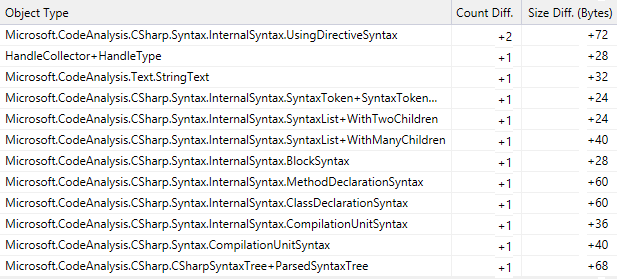
\includegraphics[scale=0.80]{performance-node-reuse-scenario1-3}
\caption{Memory impact of the second parsing session with identical trees}
\label{img:performance-node-reuse-scenario1-3}
\end{figure}

\textbf{Conclusion:} The first parsing session creates a lot of different objects but the next session only creates a relative tiny amount of new objects. An interesting aspect to note here is the kind of objects we see created in that first run (see figure \ref{img:performance-node-reuse-scenario1-2}): every token is cached when that first parsing session starts which causes a lot of initial allocations. 
When we look further down the list of allocated objects we also see caches, the parser, specific object pools, factories and a lot more. However when we now look at the second parsing session and see how it affects the heap we see none of this: there are a few new nodes representing the broad lines of the tree but no new tokens, identifiers, parsers, caches, etc have been allocated.


\item \textbf{Scenario 2:} Parsing two slightly different syntax trees

\textbf{Expectation:} Corresponding to the previous experiment, we expect a lot of allocations in the first parsing session. The second parsing session should display a slightly higher amount of newly allocated objects than in the first experiment but it should still be relatively little considering most of the allocations came from tree-independent work like populating caches and creating parsers.

\textbf{Demonstration:} 

\lstset{style=csharp, caption={Parsing two slightly different syntax trees}}
\begin{lstlisting}
internal class Experiment2
{
	public const string tree1 = @"
using System;
using System.Text;

class MyClass 
{
    void MyMethod()
    {
        int result = 2 + 2;
        Console.WriteLine(result);
    }
}";

	public const string tree2 = @"
using System;
using System.Text;

class MyClass 
{
    private string myString = ""hello"";

    void MyMethod()
    {
        int result = 2 + 2;
        Console.WriteLine(result);
    }
}";

	private static void Main(string[] args)
	{
		var obj1 = CSharpSyntaxTree.ParseText(tree1);
		var obj2 = CSharpSyntaxTree.ParseText(tree2);
	}
}
\end{lstlisting}

\textbf{Results:}

\begin{figure}[H]
\centering
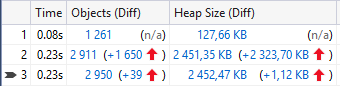
\includegraphics[scale=1]{performance-node-reuse-scenario2-1}
\caption{Memory impact comparison when parsing two slightly different syntax trees}
\label{img:performance-node-reuse-scenario2-1}
\end{figure}

\begin{figure}[H]
\centering
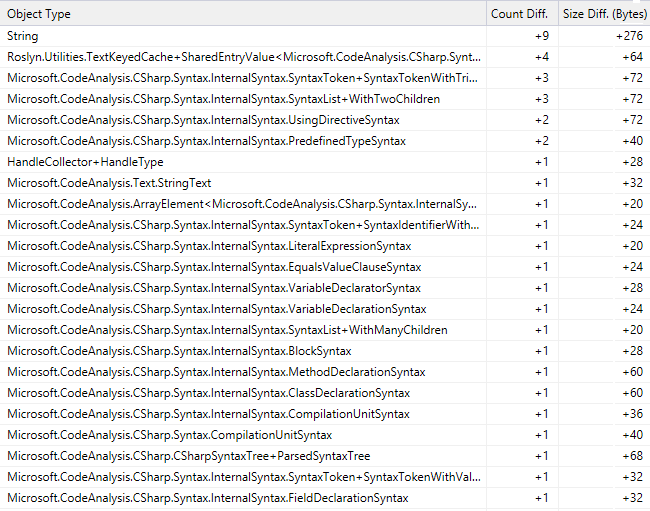
\includegraphics[scale=0.80]{performance-node-reuse-scenario2-2}
\caption{Memory impact of the second parsing session with slightly different syntax trees}
\label{img:performance-node-reuse-scenario2-2}
\end{figure}

\textbf{Conclusion:} As expected there are indeed more additional allocations in experiment 2 compared to experiment 1 (39 vs 13 respectively) which is still dwarfed by the initial allocation of 1650 objects. What we can see in figure \ref{img:performance-node-reuse-scenario2-2} are the additional string allocations and the syntax tree that makes up a field declaration (\verb|FieldDeclarationSyntax|, \verb|VariableDeclarationSyntax|, \verb|VariableDeclaratorSyntax|, and so on).

\item \textbf{Scenario 3:} Iterating through the nodes of a tree

\textbf{Expectation:} We know that red nodes are materialized lazily: they have a trivial structure when the green node is constructed and get expanded to full-fledged red nodes only when this is requested. By retrieving all the descendent nodes from the root of the tree, we expect a lot of extra allocations (relative to previous experiments). If we look at previous results we can tell they are all green nodes because the objects are contained in the \verb|InternalSyntax| namespace. By materializing, we should find allocations from objects based in the \verb|Syntax| namespace -- the red nodes that are exposed through APIs.

\textbf{Demonstration:} 

\lstset{style=csharp, caption={Iterating through the nodes of a tree}}
\begin{lstlisting}
internal class Experiment3
{
    public const string tree1 = @"
using System;
using System.Text;

class MyClass 
{
    void MyMethod()
    {
        int result = 2 + 2;
        Console.WriteLine(result);
    }
}";
    private static void Main(string[] args)
	{
		var obj1 = CSharpSyntaxTree.ParseText(tree1);
		var objects = obj1.GetRoot().DescendantNodesAndSelf()
															  .ToArray();
	}
}
\end{lstlisting}

\textbf{Results:}

\begin{figure}[H]
\centering
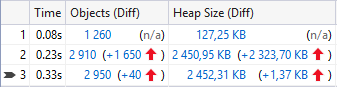
\includegraphics[scale=1]{performance-node-reuse-scenario3-1}
\caption{Memory impact comparison when materializing red nodes}
\label{img:performance-node-reuse-scenario3-1}
\end{figure}

\begin{figure}[H]
\centering
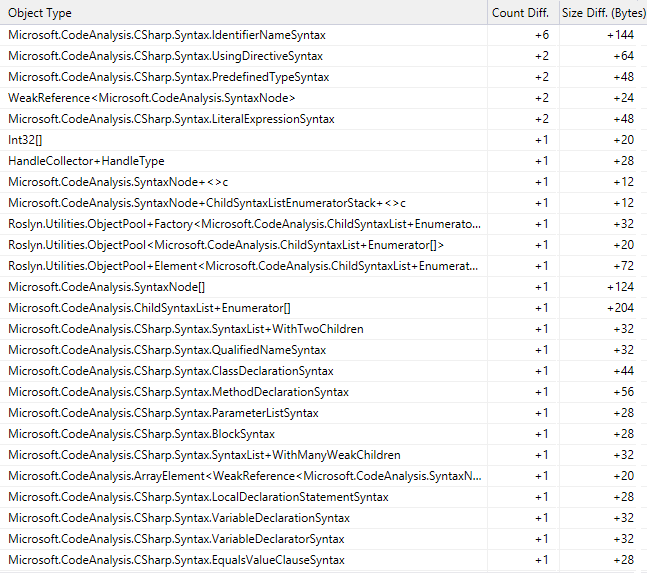
\includegraphics[scale=0.80]{performance-node-reuse-scenario3-2}
\caption{Memory impact when materializing red nodes}
\label{img:performance-node-reuse-scenario3-2}
\end{figure}

\textbf{Conclusion:} We can see that a significant amount of allocations has occurred by iterating through our syntax tree. These objects are almost all located in the \verb|Syntax| namespace which confirms our expectation that we're dealing with red nodes. It's interesting to notice that every type that existed in our green tree now created the corresponding type in the red tree. We also see the \verb|WeakReference| in play which we will discuss in section \ref{sec:weak-references}.




\end{itemize}